\section{Estudo da monotonia das funções}

\begin{frame}
    \vspace{-15pt}
    \begin{columns}
        \column{.5\textwidth}
        \begin{definition}
            Seja uma função $f$ definida em um intervalo $I$ e sejam $x_1$ e $x_2$ quaisquer números em $I$ tais que $x_1 < x_2$ então:
            \begin{itemize}
                \item<only@+> $f$ é \textbf{estritamente crescente} em $I$ se $f(x_1)<f(x_2)$.
                \item<only@+> $f$ é \textbf{estritamente decrescente} em $I$ se $f(x_1)>f(x_2)$.
                \item<only@+> $f$ é \textbf{constante} em $I$ se $f(x_1)=f(x_2)$.
            \end{itemize}
        \end{definition}
        \column{.5\textwidth}
        % FIGURAS
        \begin{figure}[H]
            \centering
            \includegraphics<1>[width=.8\linewidth]{figuras/fig1.png}
            \includegraphics<2>[width=.8\linewidth]{figuras/fig2.png}
            \includegraphics<3>[width=.8\linewidth]{figuras/fig3.png}
            % \caption{Caption}
            % \label{fig:my_label}
        \end{figure}
    \end{columns}
\end{frame}

\subsection{Teorema da monotonia}
\begin{frame}
    % \vspace{-15pt}
    \begin{theorem}[Teorema da monotonia]
        Seja $f$ contínua em um intervalo $[a,b]$ e diferenciável em $]a,b[$, então:
        \begin{itemize}
            \item Se $f'(x)>0$ para cada $x\in]a,b[$, então $f$ é \textbf{estritamente crescente} em $]a,b[$.
            \item Se $f'(x)<0$ para cada $x\in]a,b[$, então $f$ é \textbf{estritamente decrescente} em $]a,b[$.
        \end{itemize}
    \end{theorem}
    \begin{figure}
        \centering
        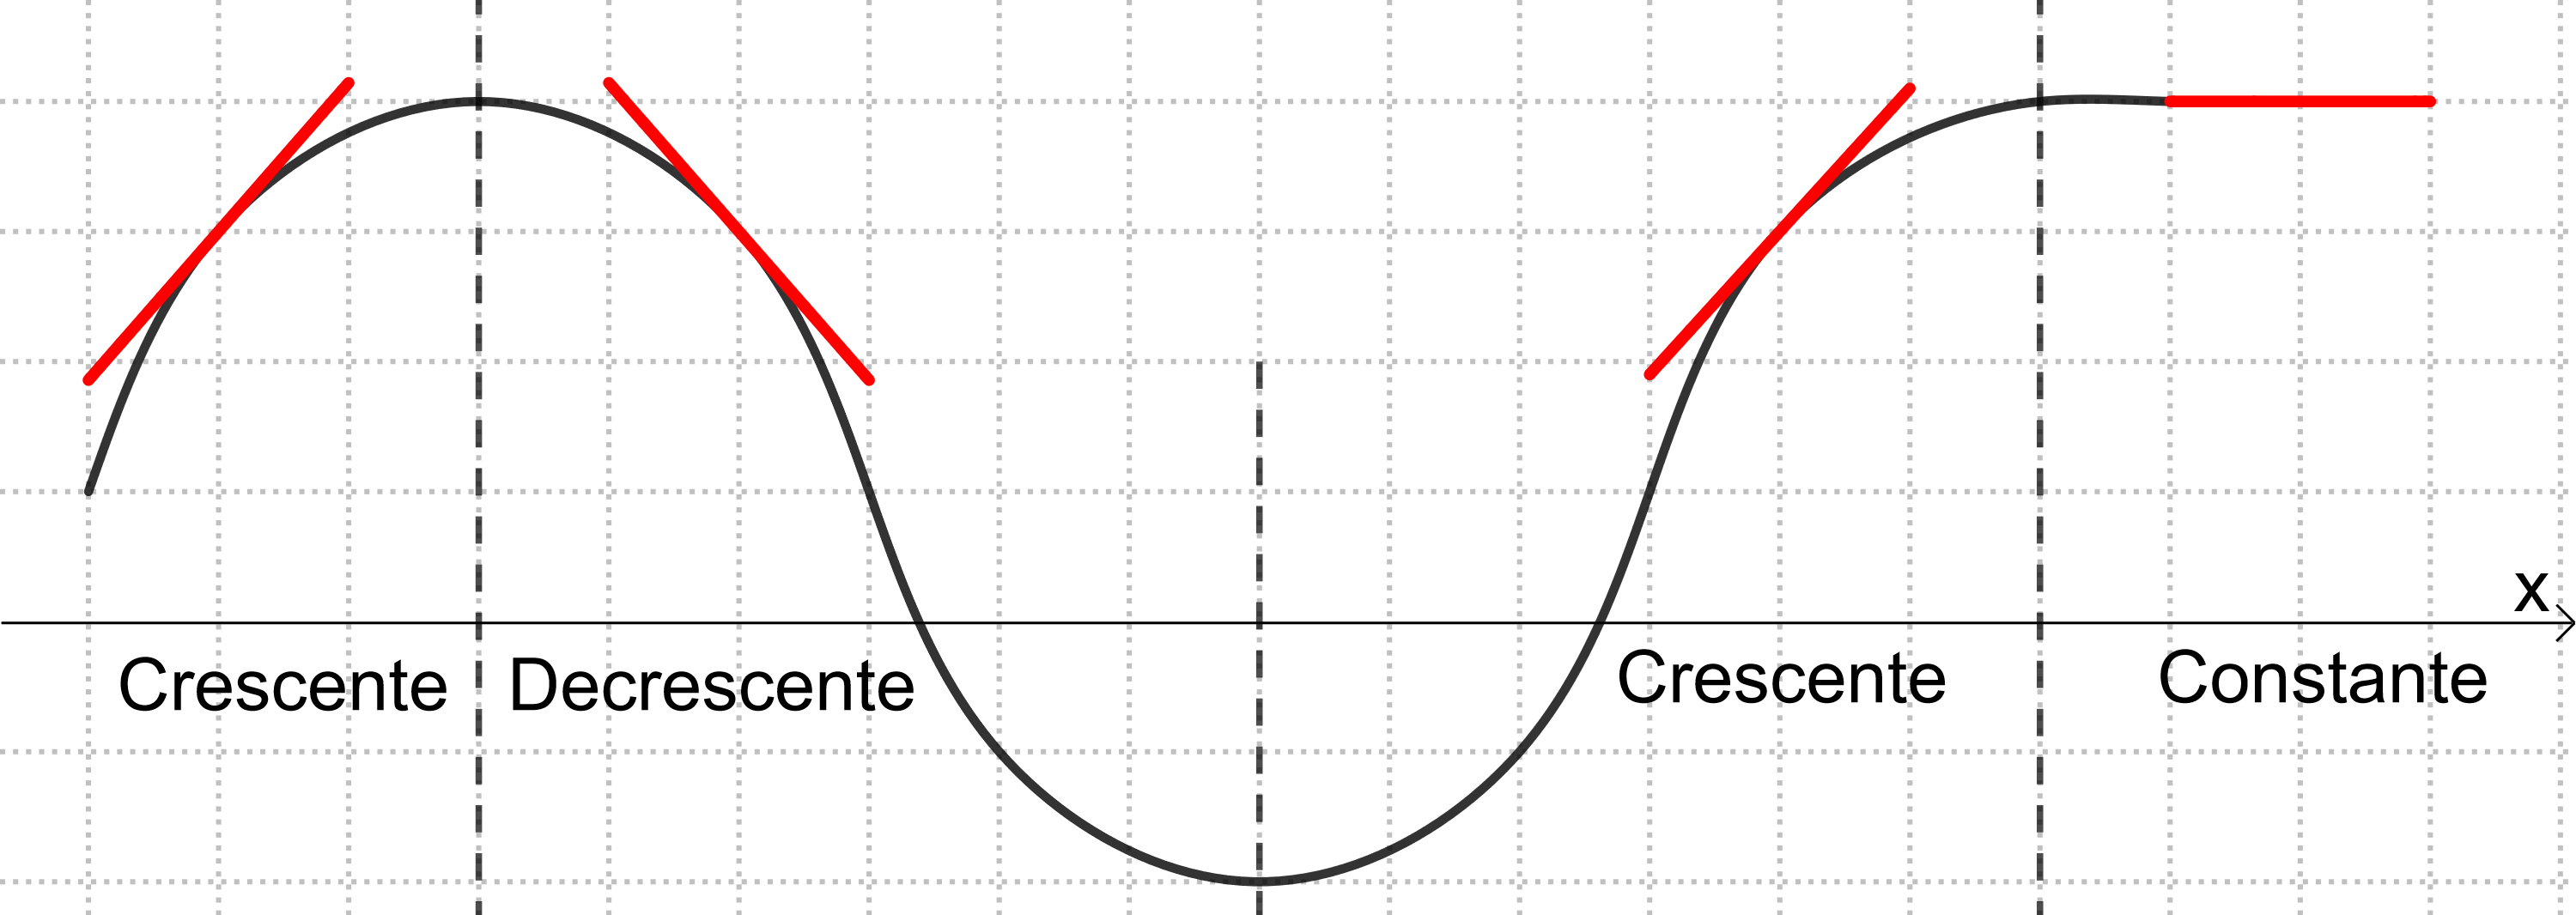
\includegraphics[width=.9\linewidth]{figuras/fig4.png}
        % \caption{Caption}
        % \label{fig:my_label}
    \end{figure}
        % FIGURAS
\end{frame}

\begin{frame}{}
    \vspace{-15pt}
    \begin{columns}
        \column{.5\textwidth}
        \begin{example}
            Determine os intervalos de crescimento e decrescimento das seguintes funções:
            \begin{enumerate}[a]
                \item<only@+> $y = x^2 +2x -3$
                \item<only@+-> $y = x + \dfrac{1}{x}$
            \end{enumerate}
    \end{example}        
        \column{.5\textwidth}
    \end{columns}

\end{frame}

\subsection{Pontos extremos}
\begin{frame}{Pontos extremos}
    \begin{theorem}
        Se $f(x)$ assume valor extremo em $x=c$ e $f(x)$ é derivável nesse ponto, então $f'(c)=0$.
    \end{theorem}
    \begin{columns}
        \column{.5\linewidth}
    \textbf{Observação.} A recíproca não é verdadeira. Por exemplo, em $f(x)=x^3$ temos $f'(0)=0$, mas $x=0$ não é um extremo.
    % FIGURA
    \begin{figure}
        \centering
        \includegraphics[width=.6\linewidth]{/figuras/exemplo-nao-ponto-extremo.png}
        % \caption{Caption}
        % \label{fig:my_label}
    \end{figure}        
        \column{.5\linewidth}
    \begin{itemize}
        \item \textbf{Máximo absoluto (ou máximo global):} é a maior imagem de uma função num intervalo.
        \item \textbf{Mínimo absoluto (ou mínimo global):} é a menor imagem de uma função num intervalo.
    \end{itemize}        
    \end{columns}


\end{frame}

\begin{frame}{}
    \begin{figure}
        \centering
        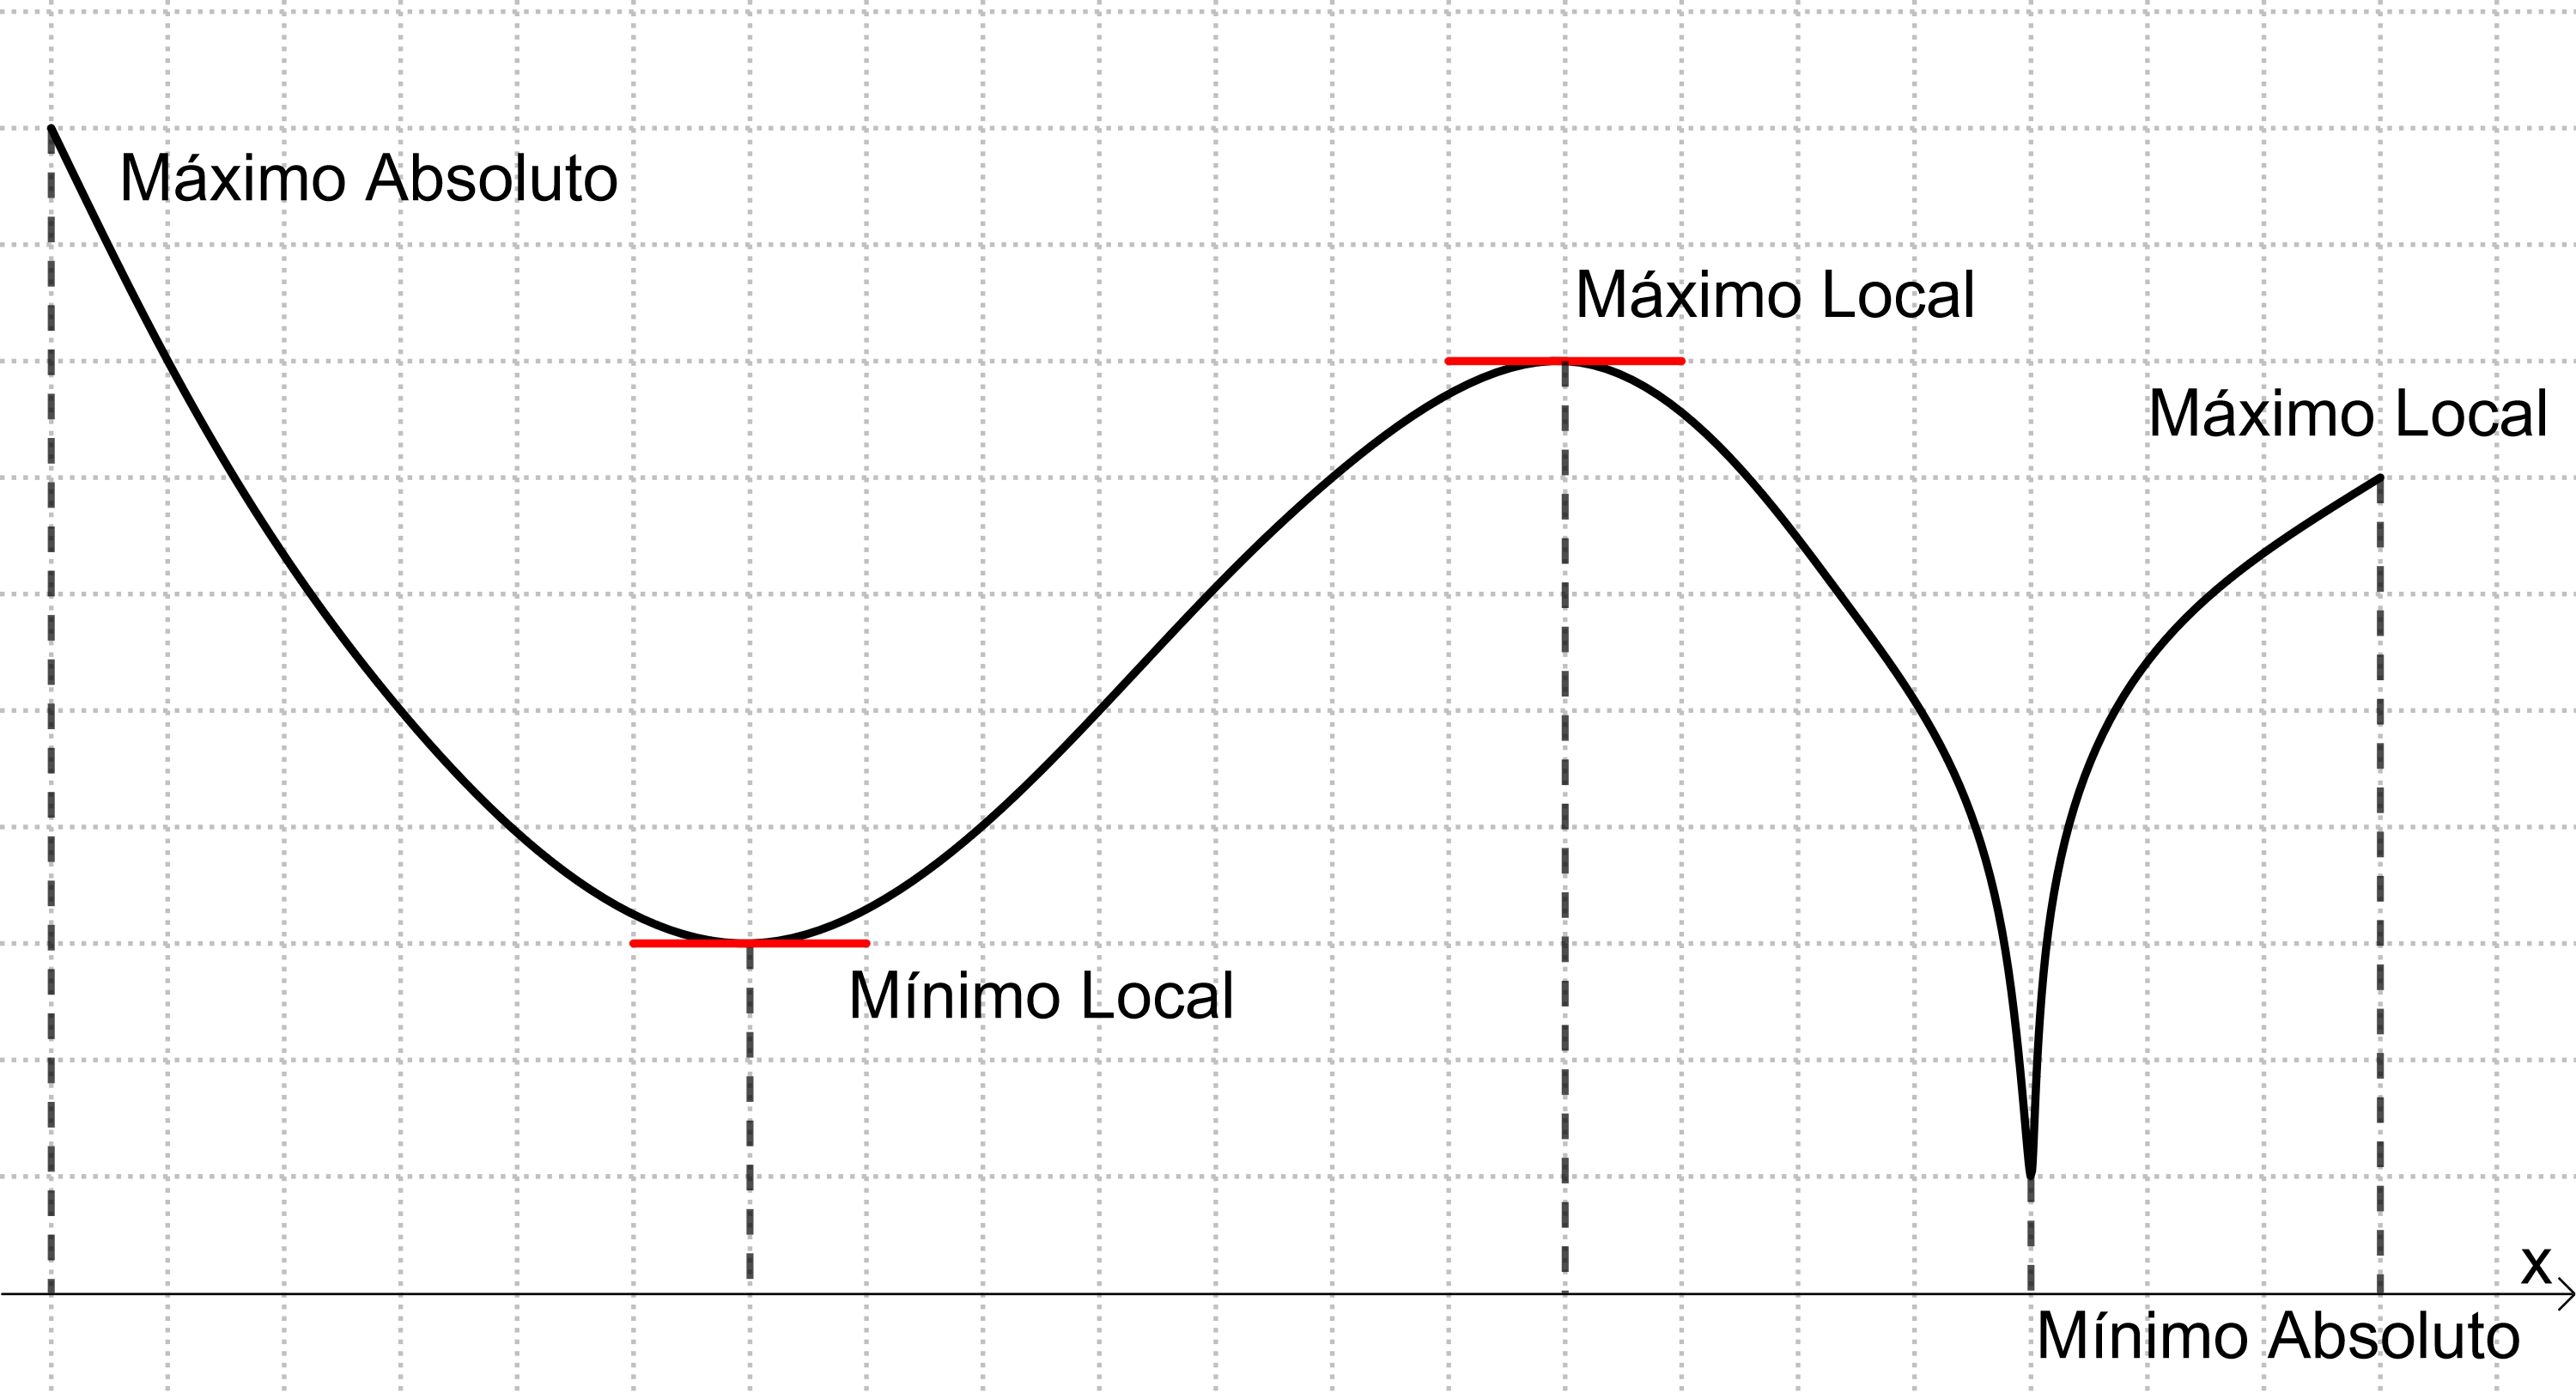
\includegraphics[width=.9\linewidth]{figuras/fig5.png}
        % \caption{Caption}
        % \label{fig:my_label}
    \end{figure}       
\end{frame}

\subsection{Pontos críticos}
\begin{frame}{Pontos críticos}
    \begin{theorem}
        O ponto $c\in D(f)$ é um \textit{ponto crítico}, se $f'(c)=0$ ou se $f'(c)$ não existe.
    \end{theorem}
    
    \begin{itemize}
        \item Uma condição necessária para a existência de um extremo relativo em um ponto $c$ é que $c$ seja ponto crítico.
    \end{itemize}
\begin{figure}
    \centering
    % \includegraphics[width=.3\textwidth]{figuras/exemplo-nao-ponto-extremo.png}
    % \hfill
    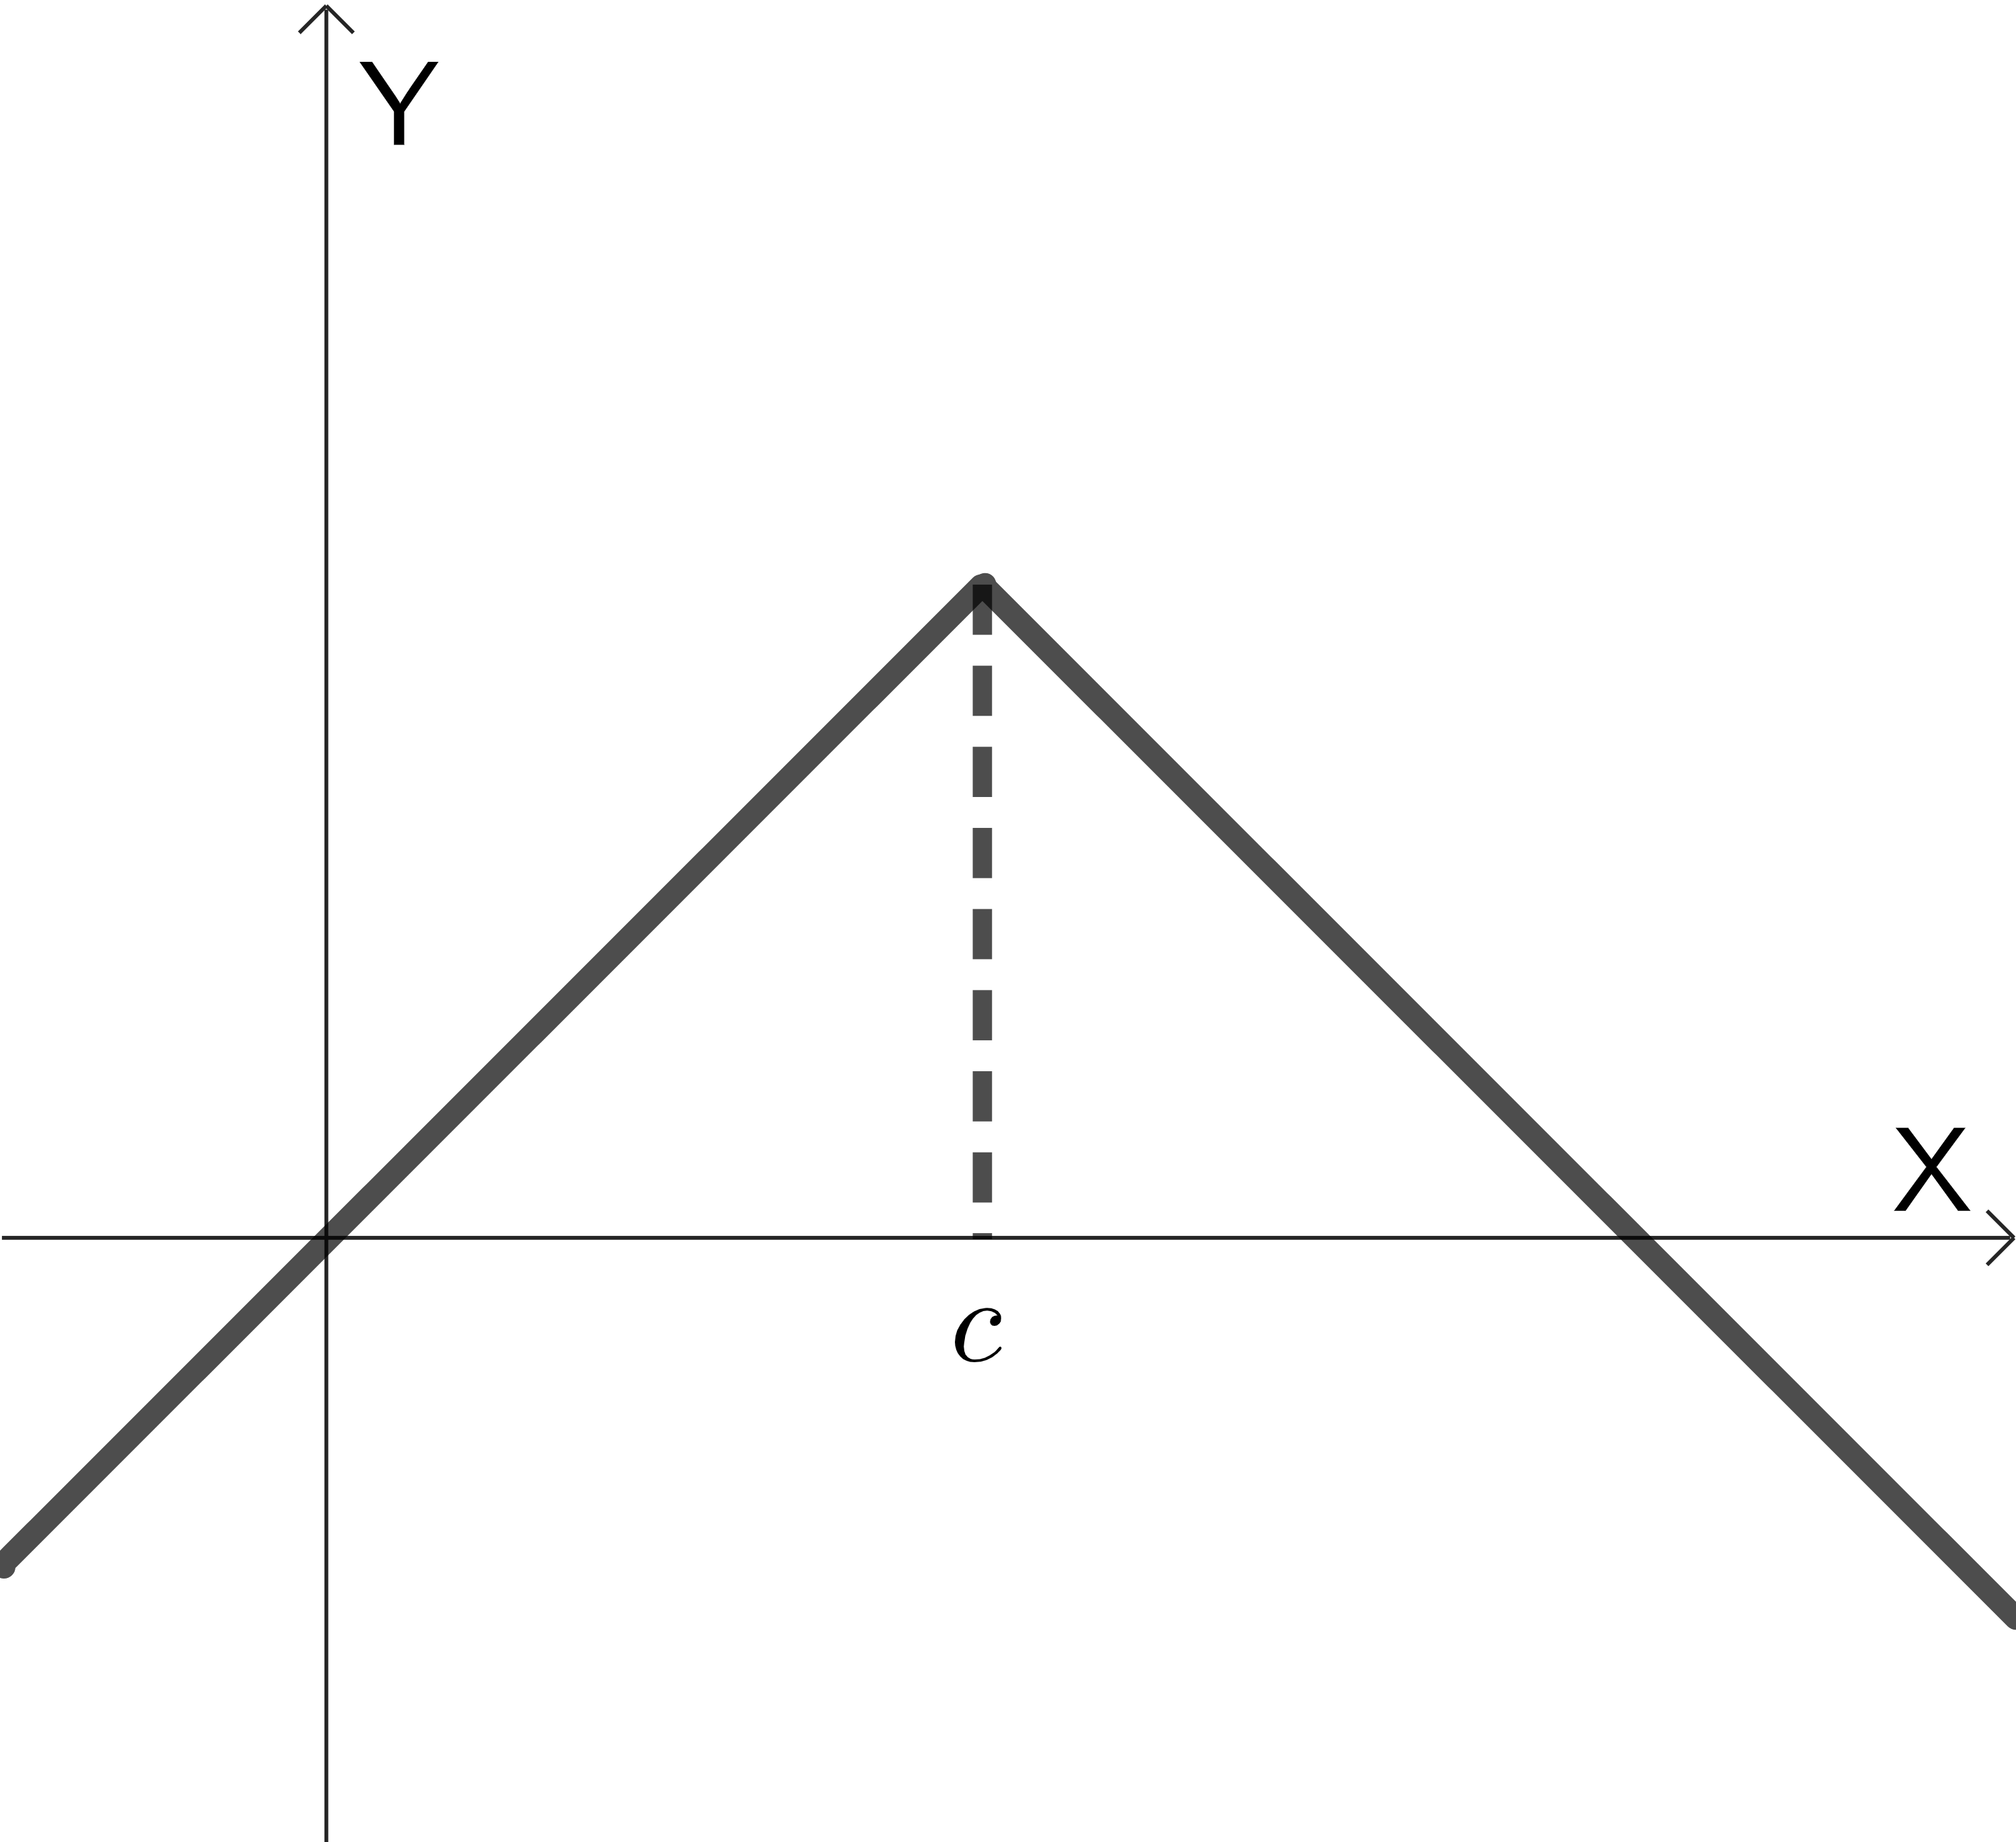
\includegraphics[width=.3\textwidth]{figuras/ex1-ponto-critico.png}
    \hspace{1cm}
    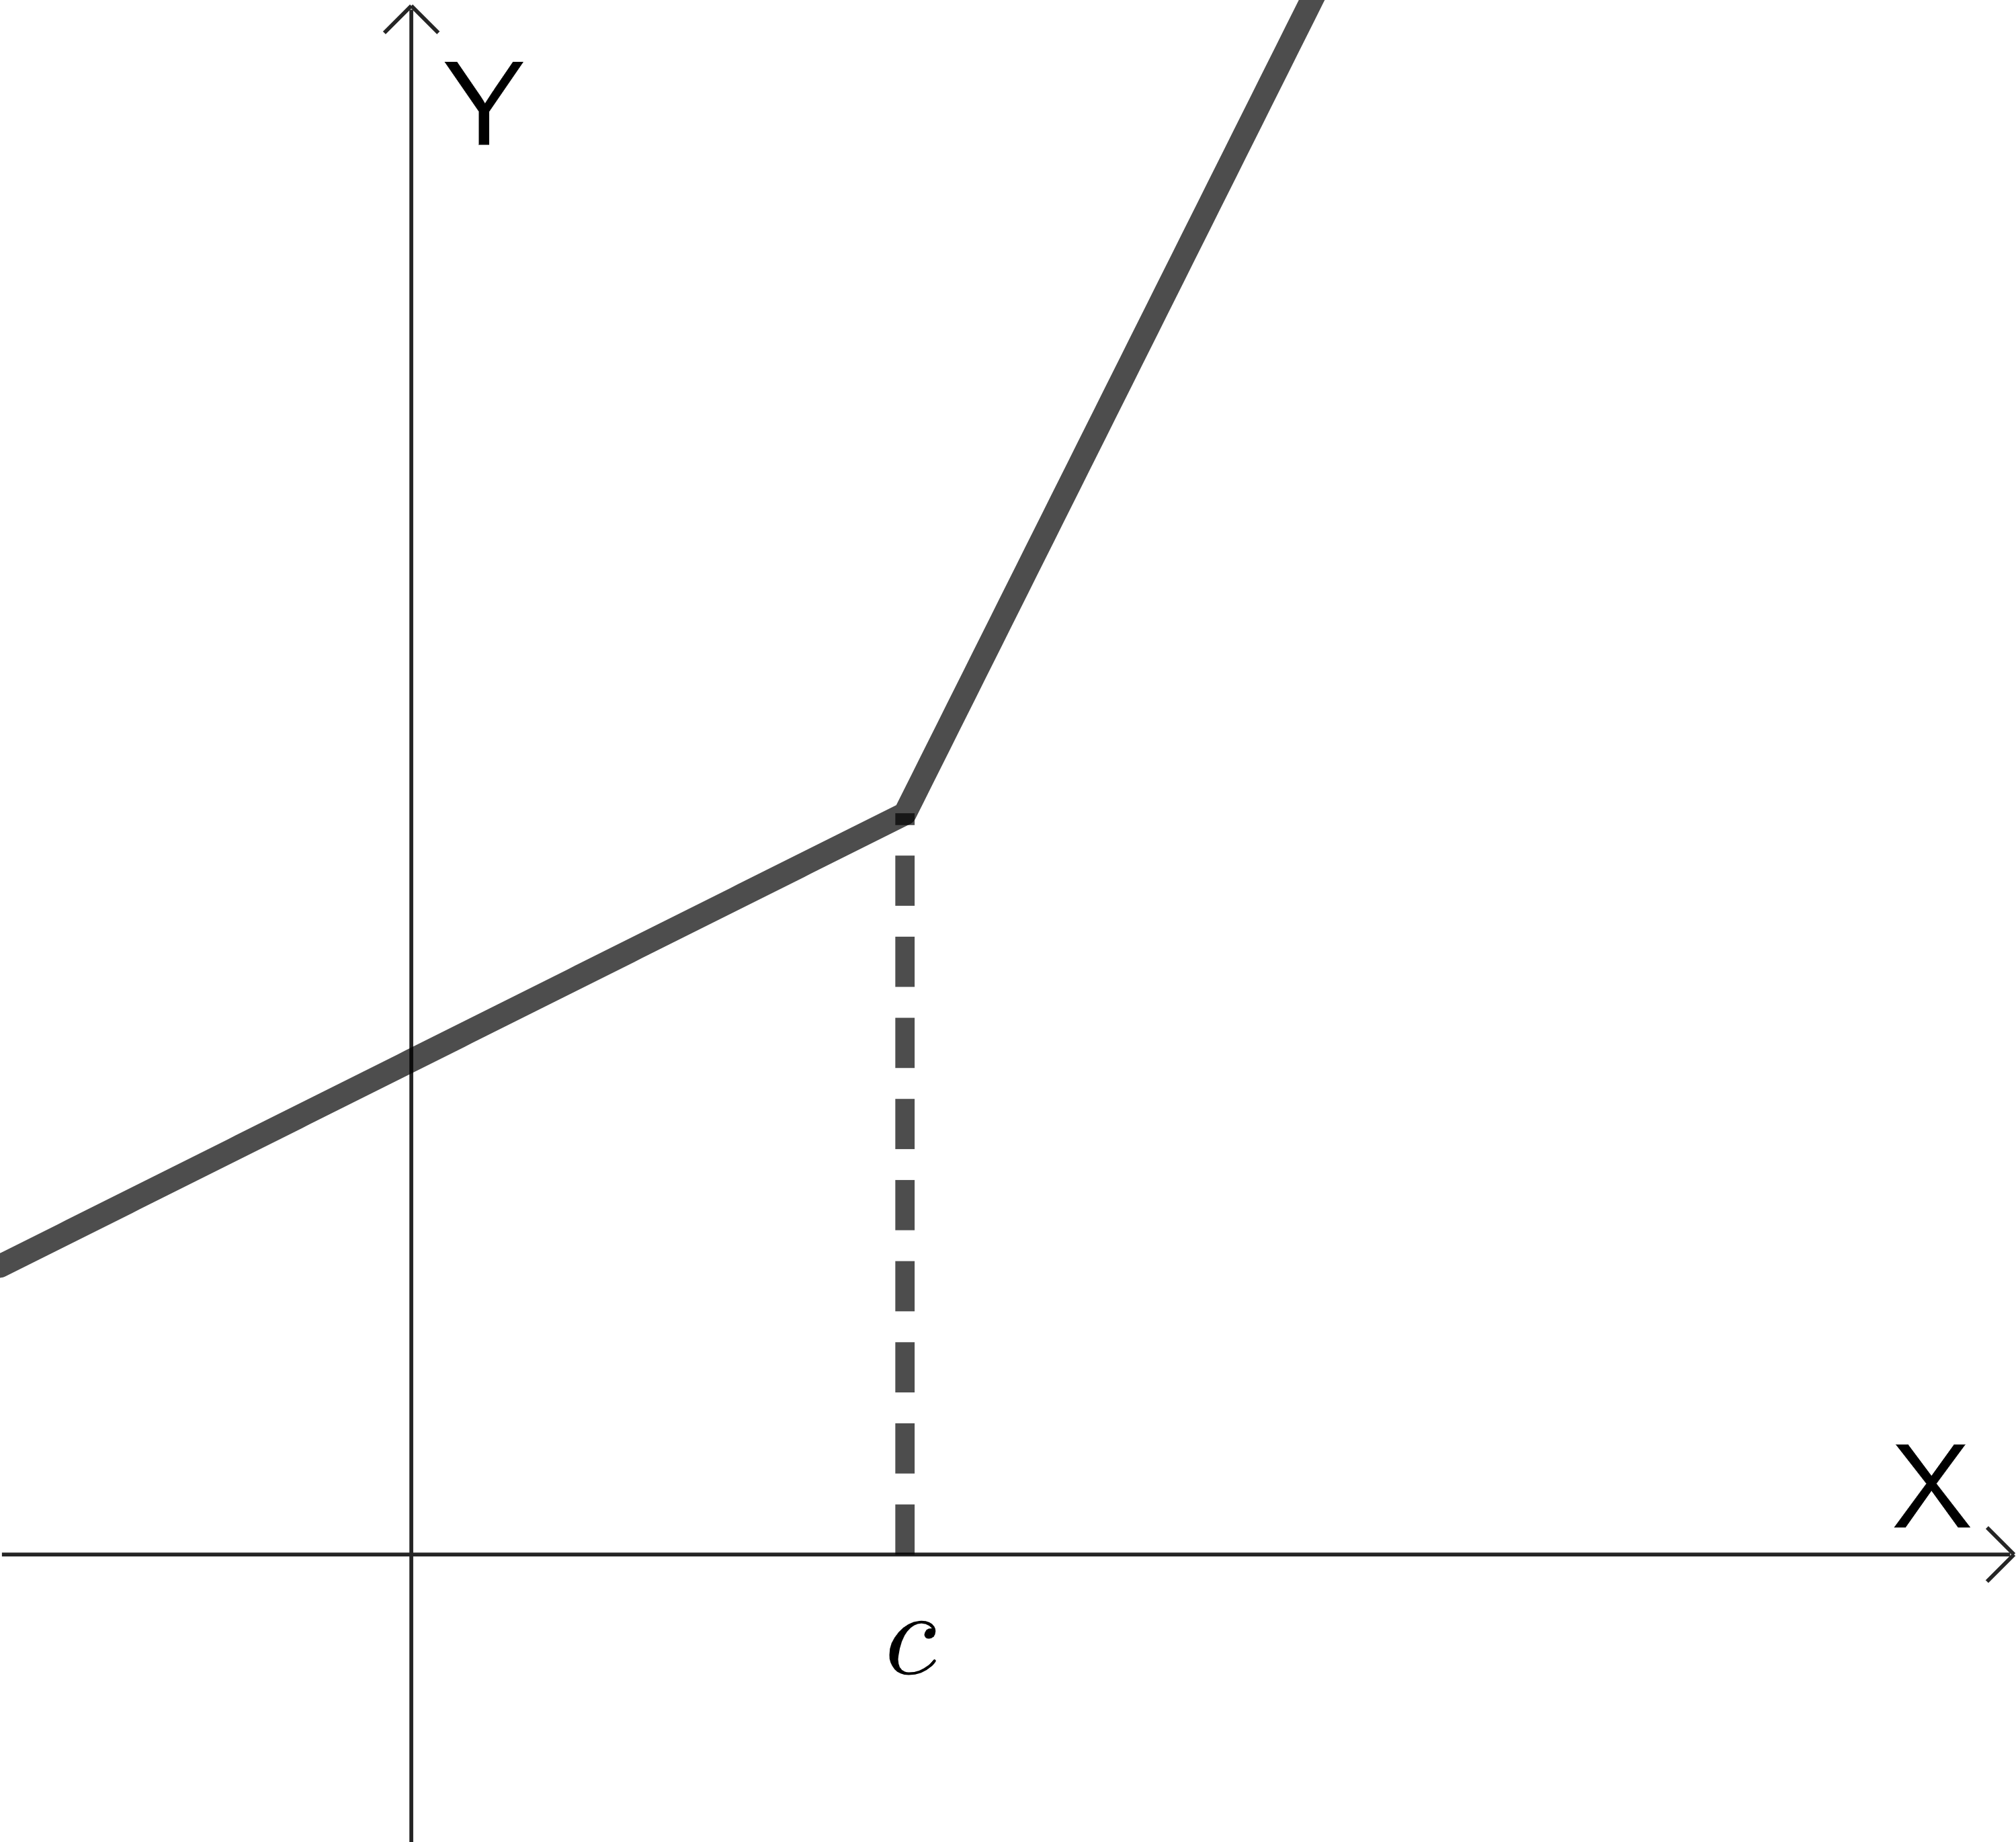
\includegraphics[width=.3\textwidth]{figuras/ex2-ponto-critico.png}
    % \caption{Caption}
    % \label{fig:my_label}
\end{figure}    
\end{frame}

\section{Teste da primeira derivada}
\begin{frame}{Teste da primeira derivada}
\begin{columns}
    \column{.5\textwidth}
\begin{theorem}
    Seja $f$ contínua num intervalo fechado $[a,b]$ e diferenciável em todo o intervalo $]a,b[$, exceto possivelmente num ponto c. 
    \begin{itemize}
        \item<only@+> Se os valores de $f'$ passam de positivos para negativos em $c$, então $f(c)$ é um \textbf{máximo local (ou máximo relativo)} de $f$.
        \item<only@+> Se os valores de $f'$ passam de negativos para positivos em $c$, então $f(c)$ é um \textbf{mínimo local (ou mínimo relativo)} de $f$.
        \item<only@+> Se $f'(x)>0$ ou se $f'(x)<0$ para todo $x$ em $]a,b[$, exceto $x=c$, então $f(c)$ \textbf{não é extremo local} de $f$.
    \end{itemize}    
\end{theorem}    
    \column{.5\textwidth}
    \begin{figure}
        \centering
        \includegraphics<1>[width=.9\linewidth]{figuras/fig6.png}
        \includegraphics<2>[width=.9\linewidth]{figuras/fig7.png}
        \includegraphics<3>[width=.9\linewidth]{figuras/fig8.png}
        % \caption{Caption}
        % \label{fig:my_label}
    \end{figure}
\end{columns}
\end{frame}

\subsection{Exemplos}
\begin{frame}{}
    \begin{example}
        Determine os extremos locais das seguintes funções:
        \begin{enumerate}[a]
            \item<only@+> $y = x^2 +2x -3$
            \item<only@+> $y = x + \dfrac{1}{x}$
        \end{enumerate}
    \end{example}
\end{frame}

\begin{frame}{}
    \begin{example}
        Considere a função definida por $f(x)=12 + 2x^2 - x^4$. Determine:
        \begin{enumerate}[a]
            \item<only@+> os intervalos de crescimento e decrescimento de $f$.
            \item<only@+> os pontos extremos.
            \item<only@+> faça um esboço do gráfico de $f$.
        \end{enumerate}
    \end{example}
\end{frame}